\chapter{Natural Language Processing}
\label{chap:nlp}

\section{Machine Learning}
\label{sec:ml}

\subsection{Textbereinigung und Vorverarbeitung}
\label{sec:text_vorverarbeitung}

\begin{itemize}
    \item \textbf{Titel und Inhalt der Artikel zusammenfügen \cite{Buddhadev2025}}: Damit keine wichtigen Informationen verloren gehen,
    werden Titel und Inhalt des Artikels zusammengefasst. Gerade der Titel kann durch z.B. Clickbait (siehe \ref{sec:wie_definieren_sich_fake_news})
    schnell Hinweise auf eventuelle Fake News geben.

    \item \textbf{Akzente und Sonderzeichen entfernen \cite{Buddhadev2025} \cite{sabir2025} \cite{aslam2022}}: Akzente führen dazu, dass Wörter wie „café“ und „cafe“ unterschiedlich behandelt werden, 
    obwohl sie semantisch gleich sind. Das Entfernen dieser erhöht die Generalisierung. Sonderzeichen stören einfache Tokenizer (z. B. bei Bag-of-Words), führen zu vielen seltenen Tokens und zu 
    überdimensionierten Vektoren (siehe \ref{sec:bag_of_words}).

    \item \textbf{Alle Buchstaben zu Kleinbuchstaben konvertieren \cite{sabir2025} \cite{SUDHAKAR2024101028} \cite{aslam2022}}: Ähnlich wie zum vorherigen Punkt
    erhöht die durchgehende Kleinschreibung aller Buchstaben die Generalisierung und verhindert somit unnötige Duplikate im Vokabular.

    \item \textbf{Leere Spalten entfernen \cite{SUDHAKAR2024101028}}: Leere Spalten enthalten keine Information. 
    Sie können bei der Vektorisierung oder Modellerstellung Fehler verursachen und werden als einfache Datenbereinigungsmaßnahme entfernt.

    \item \textbf{Kontraktionen auflösen (ans -> an das) \cite{Buddhadev2025}}: Im deutschen sind Kontradiktionen zwar nicht so häufig wie im englischen,
    sie kommen aber trotzdem vor und sollten aufgelöst werden. Dies vermeidet fragmentierte Token und verbessert die Semantik und Trennbarkeit im Modell.

    \item \textbf{Stoppwörter entfernen \cite{Buddhadev2025} \cite{sabir2025} \cite{aslam2022}}: Wörter wie „der“, „ist“, „und“ tragen wenig zur inhaltlichen Differenzierung bei. 
    Das Entfernen dieser verbessert die semantische Gewichtung relevanter Begriffe \cite{sarkar2018nlpguide}.

    \item \textbf{Rechtschreibfehler korrigieren \cite{sabir2025}}: Tippfehler führen zu seltenen Tokens und stören die Generalisierung. 
    In offiziellen Artikeln sind zwar selten Rechtschreibfehler zu finden, aber falls vorhanden, hilft die Korrektur zur Verbesserung
    der Modellqualität.

    \item \textbf{Lemmatisieren \cite{Buddhadev2025} \cite{sabir2025} \cite{aslam2022}}: Bei der Lemmatisierung werden verschiedene Wortformen auf die Grundform zurückgeführt 
    („läuft“, „lief“, „laufen“ wird zu „laufen“). So erkennt das Modell gleiche Bedeutungen trotz grammatischer Variation.

    \item \textbf{Tokenisierung \cite{sabir2025}}: In der Tokenisierung werden die Texte in einzelne Wörter oder Einheiten (Tokens) zerlegt, die für Modelle verarbeitbar sind. 
    Dies ist eine Grundvoraussetzung für alle weiteren NLP-Schritte wie TF-IDF oder Word Embeddings.
\end{itemize}

\subsubsection{Nutzung einer duale Feature-Pipeline}

Ein Problem welches das Entfernen der Akzente und Sonderzeichen und das Konvertieren aller Buchstaben zu Kleinbuchstaben mit sich bringt
ist, dass viele wichtige Hinweise zum Erkennen von Fake News verloren gehen. Wie in Kapitel \ref{sec:potenzielle_indikatoren} beschrieben,
sind fortlaufende Großschreibung, übermäßige Nutzung von Satzzeichen und falsche Zeichensetzung am Satzende potenzielle Indikatoren für Fake News.

Eine duale Feature-Pipeline kann dieses Problem lösen. Implementiert wird eine „cleaned“ Version (z.B. für inhaltliche Bedeutung) mit 
standardisierten, inhaltlichen Features und eine „rohe“ Version (z.B. für Stilmerkmale) mit stilistischen, rohen Textfeatures.

So werden semantische und stilistische Hinweise genau so genutzt wie ein Mensch es beim Lesen macht.

Die Notwendigkeit der Stilmerkmale ist aber diskutierbar. Die Datensätze werden ausschließlich aus Artikeln von offiziellen
Nachrichtenportalen zusammengesetzt. Diese schreiben meist sauber, ohne Caps-Lock oder auffällige Sonderzeichen. Stilistische Merkmale wie viele 
Ausrufezeichen, Emojis oder absichtliche Rechtschreibfehler kommen dort nicht vor – also sind sie in diesem Fall auch keine verlässlichen Fake-News-Signale.

\subsection{Merkmalextraktion}
\label{sec:merkmalextraktion}


\subsubsection{Bag-of-words}
\label{sec:bag_of_words}

Das Bag-of-Words-Modell ist ein einfaches Verfahren zur Textrepräsentation, bei dem ein Dokument als Vektor der Häufigkeiten 
einzelner Wörter dargestellt wird – unabhängig von deren Reihenfolge oder Kontext. Es zählt lediglich das Vorkommen jedes Wortes aus 
einem festen Vokabular \cite{cichosz2018forum}.

\subsubsection{TF-IDF}

TF-IDF ist ein gewichtetes Modell zur Textdarstellung, das berücksichtigt, wie häufig ein Wort in einem Dokument vorkommt (TF) 
und wie selten es im gesamten Kontext ist (IDF). Es dient dazu, häufige, aber wenig informative Wörter zu reduzieren und 
aussagekräftige Begriffe zu betonen \cite{elov2023uzbek}.

\paragraph{Sparse Matrizen} werden sowohl von Bag-of-Words als auch von TF-IDF genutzt. Eine Matrix wird als sparse bezeichnet, 
wenn der Anteil der Nicht-Null-Werte im Verhältnis zur Gesamtanzahl der Dokumente sehr klein ist. Pro hinzugefügtem Dokument wird eine Zeile 
erstellt und pro Wort im Vokabular eine Spalte. Da jedes Dokument nur einen Bruchteil der Wörter des Gesamtvokabulars enthält, bestehen
der Großteil einer solchen Matrix aus Nullen.

\begin{figure}[h]
    \begin{subfigure}{0.5\textwidth}
        \centering
        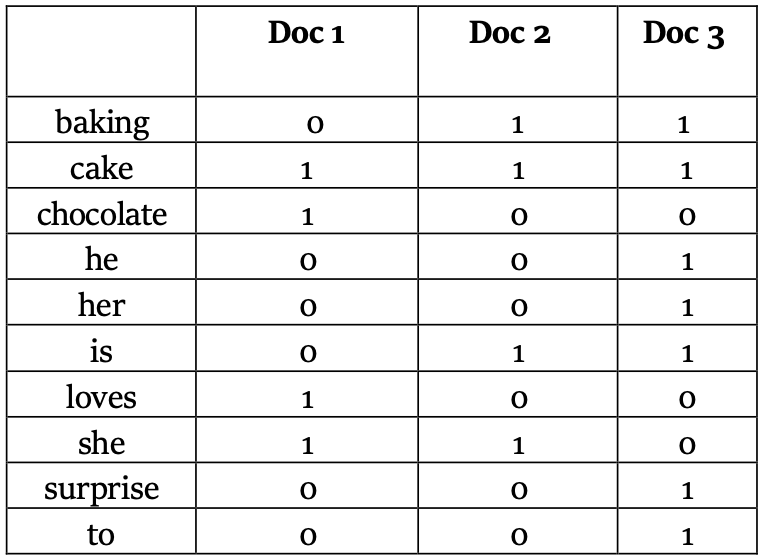
\includegraphics[scale=0.5]{static/table_bow.png}
        \caption{\label{fig:table_bow} Bag-of-words Sparse Matrix \cite{Buddhadev2025}}
    \end{subfigure}
    \begin{subfigure}{0.5\textwidth}
        \centering
        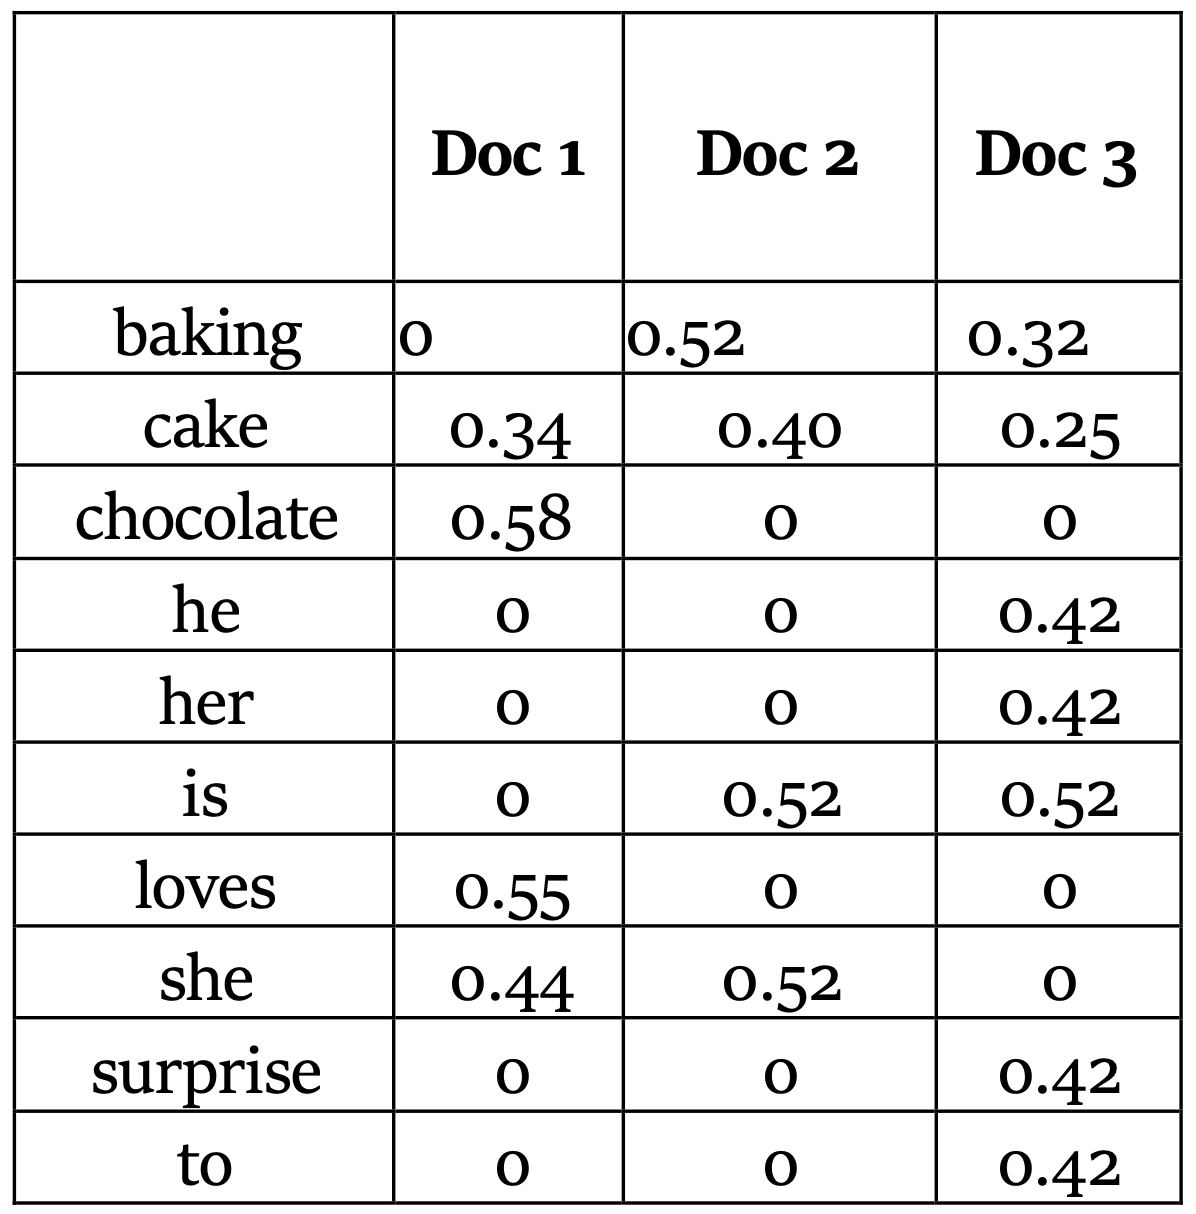
\includegraphics[scale=0.25]{static/table_tf-idf.png}
        \caption{\label{fig:table_tf-idf} TF-IDF Sparse Matrix \cite{Buddhadev2025}}
    \end{subfigure}
    
    \caption{Vergleich der Sparse Matrizen}
    \label{fig:vlg_sparse_matrizen}
\end{figure}

In Abbildung \ref{fig:vlg_sparse_matrizen} wurden den beiden Matrizen jeweils die drei Dokumente:

\begin{itemize}
    \item Doc1 - She loves chocolate cake
    \item Doc2 - She is baking a cake
    \item Doc3 - He is baking a cake to surprise her
\end{itemize}

hinzugefügt. In der Matrix \ref{fig:table_bow} werden in jeder Zelle in welcher das Dokument das entsprechende Wort beinhaltet eine 1 gesetzt.
In \ref{fig:table_tf-idf} wird statt einer 1 eine Gewichtung über die Häufigkeit der Wörter in allen Dokumenten hinweg erstellt und eingetragen.
Sie bewertet die Wichtigkeit eines Wortes in einem Dokument relativ zur gesamten Sammlung von Dokumenten. Dabei wird die Termfrequenz (TF) mit der 
invertierten Dokumentfrequenz (IDF) multipliziert. Je höher der resultierende Wert, desto relevanter ist das Wort für das jeweilige Dokument. 
Die Formel lautet:

\begin{equation}
    \text{tfidf}(t, d, D) = \text{tf}(t, d) \cdot \text{idf}(t, D)
\end{equation}

Dabei ist \( t \) das Wort, \( d \) das Dokument und \( D \) die gesamte Dokumentensammlung \cite{aslam2022}.

Die TF misst, wie häufig ein bestimmter Begriff \( t \) in einem Dokument \( d \) vorkommt. 
Sie beschreibt die lokale Bedeutung eines Wortes innerhalb des Dokuments.

\begin{equation}
\text{tf}(t, d) = \frac{\text{Anzahl der Vorkommen von } t \text{ in } d}{\text{Gesamtanzahl der Wörter in } d}
\end{equation}

Die IDF bewertet, wie selten ein Begriff \( t \) in der gesamten Dokumentensammlung \( D \) ist. 
Je seltener ein Begriff in vielen Dokumenten vorkommt, desto höher ist sein IDF-Wert.

\begin{equation}
    \text{idf}(t, D) = \log \left( \frac{N}{\text{df}(t)} \right)
\end{equation}

Dabei ist \( N \) die Gesamtanzahl der Dokumente in der Matrix und \( \text{df}(t) \) die Anzahl der Dokumente, 
in denen der Begriff \( t \) vorkommt \cite{qaiser2018}.

Die in \cite{Domenico2016} beschriebene Relevance Frequency (RF) ist eine überwachte Gewichtungsform der IDF-Komponente im TF-IDF, die nicht nur zählt, 
in wie vielen Dokumenten ein Begriff vorkommt, sondern berücksichtigt, in welchen Klassen der Begriff besonders häufig oder exklusiv ist.
Die Formel lautet:

\begin{equation}
    \text{rf}(t) = \log\left(2 + \frac{P(t)}{\max(1, N(t))} \right)
\end{equation}

Mit \( P(t) \) für die Anzahl der relevanten Dokumente (z.\,B. positive Klasse), in denen der Term \( t \)
und \( N(t) \) für die Anzahl der irrelevanten Dokumente (z.\,B. negative Klasse), in denen der Term \( t \) vorkommt.

Während klassisches IDF ein Wort umso höher gewichtet, je seltener es allgemein in der Gesamtmatrix ist,
gewichtet RF hingegen ein Wort umso höher, je stärker es mit einer bestimmten Zielklasse assoziiert ist.
Dadurch hebt RF Begriffe hervor, die klassenunterscheidend sind was beim Arbeiten mit überwachten Modellen relevant ist.

In der IF-IDF wird für IDF wird nun also RF eingesetzt und es ergibt sich folgende Formel:

\begin{equation}
    \text{tfidf}(t, d) = \frac{\text{Anzahl der Vorkommen von } t \text{ in } d}{\text{Gesamtanzahl der Wörter in } d} \cdot \log\left(2 + \frac{P(t)}{\max(1, N(t))} \right)
\end{equation}

\begin{itemize}
    \item Mit dem Wort \( t \) und dem Dokument \( d \) 
    \item \( P(t) \) für die Anzahl der relevanten Dokumente (z.\,B. positive Klasse), in denen der Term \( t \) vorkommt
    \item \( N(t) \) für die Anzahl der irrelevanten Dokumente (z.\,B. negative Klasse), in denen der Term \( t \) vorkommt
\end{itemize}

\subsubsection{Vergleich Bag-of-words und TF-IDF}

\begin{table}[!ht]
    \centering
        \begin{tabular}{|p{6cm}|p{6cm}|}
            \hline
            \textbf{Bag-of-Words (BoW)} & \textbf{TF-IDF} \\
            \hline
            Einfache Implementierung \cite{cichosz2018forum} & Berücksichtigt Wortwichtigkeit in gesamter Matrix  \cite{elov2023uzbek} \\
            \hline
            Keine Gewichtung — häufige Wörter dominieren & Seltener, aber informativer Inhalt wird stärker gewichtet \cite{das2023tfidf} \\
            \hline
            Hohe Dimensionalität (Sparse Matrix) & Gleiches Problem, aber mit informativeren Werten \cite{alzami2020tfidf} \\
            \hline
            Ignoriert Wortreihenfolge und Kontext \cite{umar2022sentiment} & Gleiches Grundproblem, aber geringfügig bessere Performance \cite{parmar2024stacking} \\
            \hline
            Nützlich für einfache Klassifikatoren & Bessere Klassifikationsergebnisse in Kombination mit SVM oder Logistic Regression \cite{iyer2024sentiment} \\
            \hline
        \end{tabular}
    \caption{Vergleich der Vor- und Nachteile von BoW und TF-IDF}
    \label{tab:vergleich}
\end{table}

Aus \ref{tab:vergleich} zu erkennen ist, dass TF-IDF in vielen Anwendungen leistungsfähiger ist als BoW. Insbesondere bei Texten mit hohem Vokabularumfang.

\subsubsection{Hashing Vectorizer}

Ein Hashing Vectorizer ist eine Methode zur Umwandlung von Text in numerische Merkmalsvektoren, ohne dass ein Vokabular explizit 
erstellt oder gespeichert wird. Stattdessen wird eine Hash-Funktion verwendet, um jedes Wort auf einen Index im Feature-Vektor abzubilden \cite{Buddhadev2025}.

In Abbildung \ref{fig:vgl_bow_tfidf_hashing} wird der Vergleich zwischen Machine-Learning-Modellen unter Verwendung von BoW-, TF-IDF- und
Hashing-Features gezeigt. Die y-Achse präsentiert den F1-Score, also die Precision und Recall-Werte der jeweiligen Modelle.
Das Random-Forest-Modell (RF) zeigt eine schwache Leistung bei der Verwendung von Hashing, während die linearen Modelle 
(z.B. SVM (Support Vector Machine) und LR (Logistische Regression)) ihre F1-Werte mit Hashing-Features verbessern konnten. 

Die Verbesserung ist aber nur minimal. Der F1-Score bei SVM ist ohne Hashing bei 0.89 und nach bei 0.90. 
Bei LR steigt der Wert auch von 0.87 und 0.88.

\begin{figure}[htbp]
    \begin{center}
        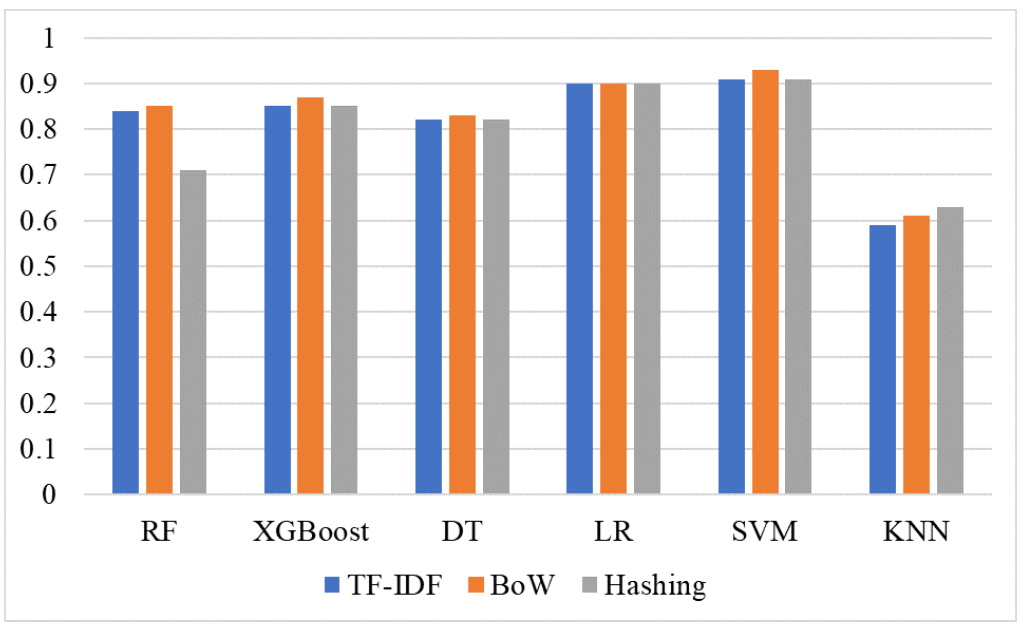
\includegraphics[scale=0.5]{static/bow_vs_tfidf_vs_hashing.png}
        \caption{\label{fig:vgl_bow_tfidf_hashing} Vergleich verschiedener Modelle mit BoW, TF-IDF und Hashing \cite{aslam2022}}
    \end{center}
\end{figure}

\subsection{Machine Learning Modelle}
\label{sec:ml_modelle}

\subsubsection{Naive Bayes}



\subsubsection{Support Vector Machines}

\subsubsection{Logistische Regression}


\section{Deep Learning}
\label{sec:deep_learning}

\subsection{Word Embeddings}
\label{sec:word_embeddings}

\subsubsection{Word2Vec}

\subsubsection{GloVe}

\subsubsection{BERT-Tokenisierung}


\subsection{Deep Learning-Modelle}
\label{sec:deep_learning_modelle}

\subsubsection{CNN}

\subsubsection{LSTM}

\subsubsection{Transformer: BERT}


\section{Hybride Modelle}
\label{sec:hybride_modelle}

\subsection{convolutional neural network (CNN) along with bi-directional LSTM}

\cite{Buddhadev2025}

% \section{Diskussion: White Box vs. Black Box-Ansätze zur Erklärbarkeit}
% \label{sec:diskussion_erklaerbarkeit}